% Лабораторная работа №3. Интерполяционный кубический сплайн.

\documentclass[a4paper, final]{article}

% ============================================================
% settings
% ============================================================
\usepackage[russian]{babel}
\usepackage{fontspec}
\setmainfont{Times New Roman}
\newfontfamily\cyrillicfonttt{Courier New}
\usepackage[14pt]{extsizes}
\usepackage[left=20mm, top=20mm, right=20mm, bottom=20mm, footskip=10mm]{geometry}
\usepackage{ragged2e}
\usepackage{indentfirst}
\usepackage{graphicx}
\usepackage{tikz}
\usepackage{caption}
\usepackage{xcolor}
\usepackage{subcaption}
\usepackage{listings}
\usetikzlibrary{arrows.meta}
\usepackage{nccmath}
\usepackage{soul}
\usepackage{algorithm}
\usepackage{algorithmic}
\usepackage{booktabs}
\usepackage{hyperref}
\usepackage{pdflscape}
\usepackage{amsmath}

\definecolor{link_color}{HTML}{0000EE}

\hypersetup{
    colorlinks=true,
    linkcolor=link_color,
    urlcolor=link_color,
    citecolor=link_color
}

\lstset{
    language=Python,
    basicstyle=\cyrillicfonttt\small,
    numbers=left,
    numberstyle=\tiny\color{gray},
    keywordstyle=\color{blue}\bfseries,
    commentstyle=\color{gray}\itshape,
    stringstyle=\color{red},
    frame=single,
    captionpos=b,
    breaklines=true,
    breakatwhitespace=false,
    showstringspaces=false,
    keepspaces=true,
    columns=flexible,
    fontadjust=true,
    basewidth={0.5em,0.45em},
    tabsize=4,
}

\begin{document}

% ============================================================
% title
% ============================================================
{
\thispagestyle{empty}
\begin{center}
    \hfill \break
    \hfill \break
    МИНИСТЕРСТВО НАУКИ И ВЫСШЕГО ОБРАЗОВАНИЯ РОССИЙСКОЙ ФЕДЕРАЦИИ\\[5 pt]
    Федеральное государственное автономное образовательное учреждение высшего образования
    «Санкт-Петербургский политехнический университет Петра Великого»\\[10 pt]
    Институт компьютерных наук и кибербезопасности\\[5 pt]
    Направление: 02.03.01 Математика и компьютерные науки\\[30pt]


    {\large Отчет по дисциплине: «Вычислительная математика»}\\[30 pt]
    \LARGE\bf «Лабораторная работа №3».
\end{center}

\vspace{110 pt}

\begin{tabular*}{460pt}{@{\extracolsep{\fill}} l r}
     Студент,\tabularnewline группы 5130201/40003 \hspace{50pt}&  \line(1,0){100} \quad Адиатуллин Т. Р.\\
     & \\
     Руководитель,\tabularnewline Преподаватель & \line(1,0){121,5} \quad Пак В. Г.\\
     & \\
     & \\
     & \\
     & \guillemotleft \line(1,0){30} \guillemotright \line(1,0){100} \, 2026 \,г.

\end{tabular*} \\

\vfill

\begin{center}
    Санкт-Петербург, 2026
\end{center}
\newpage
}

\tableofcontents
\newpage

% ============================================================
% task
% ============================================================
\section{Постановка задачи}

\textbf{Тема:} кубические сплайны.

\textbf{Цель:} научиться строить интерполяционные кубические сплайны для
табличных функций.

\textbf{Задание:} построить для данной табличной функции интерполяционный
кубический сплайн дефекта 1 с заданными граничными условиями. Коэффициенты
вычислять с четырьмя знаками после запятой в мантиссе. Проверить все условия,
налагаемые на сплайн.

\textbf{Вариант 1.} Таблица значений функции приведена в
таблице~\ref{tab:source}. Граничные условия — заданные значения производных
функции в крайних точках, причём производные вычисляются по формулам
односторонних разностных производных.

\begin{table}[h!]
\centering
\begin{tabular}{|c|c|c|c|c|c|c|c|c|c|}
\hline
$i$   & 0 & 1 & 2 & 3 & 4 & 5 & 6 & 7 & 8 \\
\hline
$x_i$ & 0,698 & 0,706 & 0,714 & 0,727 & 0,736 & 0,747 & 0,760 & 0,769 & 0,782 \\
\hline
$y_i$ & 2,2234 & 2,2438 & 2,2645 & 2,2984 & 2,3222 & 2,3516 & 2,3869 & 2,4116 & 2,4478 \\
\hline
\end{tabular}
\caption{Исходные данные функции $y = f(x)$.}
\label{tab:source}
\end{table}

Интерполяционным кубическим сплайном $S(x)$ дефекта 1 называется функция,
удовлетворяющая следующим условиям:
\begin{enumerate}
    \item на каждом частичном отрезке $[x_{i-1}, x_i]$, $i = 1, \ldots, 8$,
          $S(x)$ совпадает с некоторым кубическим многочленом $P_{3,i}(x)$;
    \item $S(x_i) = y_i$ для всех $i = 0, \ldots, 8$ (условия интерполяции);
    \item $S(x) \in C^{2}[x_0, x_8]$, т.\,е.\ сплайн и его производные первого и
          второго порядка непрерывны на всём отрезке.
\end{enumerate}

Обозначим шаги таблицы $h_i = x_i - x_{i-1}$, $i = 1, \ldots, 8$. На каждом
частичном отрезке $[x_{i-1}, x_i]$ сплайн определяется интерполяционной
формулой Эрмита
\begin{multline}
S_3(x) = P_{3,i}(x) =
y_{i-1}\frac{(x - x_i)^2\left(2(x - x_{i-1}) + h_i\right)}{h_i^3}
+ s_{i-1}\frac{(x - x_i)^2 (x - x_{i-1})}{h_i^2} + \\
+ y_i\frac{(x - x_{i-1})^2\left(2(x_i - x) + h_i\right)}{h_i^3}
+ s_i\frac{(x - x_{i-1})^2 (x - x_i)}{h_i^2}.
\label{eq:hermite}
\end{multline}
где $s_i = S'(x_i)$ — подлежащие нахождению наклоны. Формула~\eqref{eq:hermite}
обеспечивает непрерывность самого сплайна и его первой производной;
непрерывность второй производной во внутренних узлах даёт систему уравнений
\begin{equation}
\frac{1}{h_i}\, s_{i-1} + 2\!\left(\frac{1}{h_i} + \frac{1}{h_{i+1}}\right)\! s_i
+ \frac{1}{h_{i+1}}\, s_{i+1}
= 3\!\left(\frac{y_i - y_{i-1}}{h_i^{\,2}} + \frac{y_{i+1} - y_i}{h_{i+1}^{\,2}}\right),
\label{eq:system}
\end{equation}
$i = 1, \ldots, 7$. Система~\eqref{eq:system} содержит 7 уравнений и 9
неизвестных; недостающие два уравнения дают граничные условия
$s_0 = f'(x_0)$, $s_8 = f'(x_8)$.

\newpage

% ============================================================
% task1: boundary derivatives
% ============================================================
\section{Вычисление граничных производных}

Значения $f'(x_0)$ и $f'(x_8)$ оценим по простейшим односторонним разностным
формулам: правой разностью для левого конца и левой разностью для правого,
\[
f'(x_0) \approx \frac{y_1 - y_0}{h_1}, \qquad
f'(x_8) \approx \frac{y_8 - y_7}{h_8}.
\]

Подставляя табличные значения:
\begin{align*}
s_0 &= \frac{2{,}2438 - 2{,}2234}{0{,}0080} = 2{,}5500, \\[2pt]
s_8 &= \frac{2{,}4478 - 2{,}4116}{0{,}0130} = 2{,}7846.
\end{align*}

Шаги таблицы сведены в таблицу~\ref{tab:steps}.

\begin{table}[h!]
\centering
\begin{tabular}{|c|c|c|c|c|c|c|c|c|}
\hline
$i$   & 1 & 2 & 3 & 4 & 5 & 6 & 7 & 8 \\
\hline
$h_i$ & 0,0080 & 0,0080 & 0,0130 & 0,0090 & 0,0110 & 0,0130 & 0,0090 & 0,0130 \\
\hline
\end{tabular}
\caption{Шаги таблицы $h_i = x_i - x_{i-1}$.}
\label{tab:steps}
\end{table}

\newpage

% ============================================================
% task2: solve the system
% ============================================================
\section{Решение системы для наклонов}

С учётом известных $s_0$ и $s_8$ система~\eqref{eq:system} сводится к системе
из 7 линейных уравнений относительно неизвестных $s_1, \ldots, s_7$. Она
записывается в матричном виде $As = b$, где
\[
A = \begin{pmatrix}
500{,}0000 & 125{,}0000 & 0 & 0 & 0 & 0 & 0 \\
125{,}0000 & 403{,}8462 & 76{,}9231 & 0 & 0 & 0 & 0 \\
0 & 76{,}9231 & 376{,}0684 & 111{,}1111 & 0 & 0 & 0 \\
0 & 0 & 111{,}1111 & 404{,}0404 & 90{,}9091 & 0 & 0 \\
0 & 0 & 0 & 90{,}9091 & 335{,}6643 & 76{,}9231 & 0 \\
0 & 0 & 0 & 0 & 76{,}9231 & 376{,}0684 & 111{,}1111 \\
0 & 0 & 0 & 0 & 0 & 111{,}1111 & 376{,}0684
\end{pmatrix}\!
\]

\[b = \begin{pmatrix}
1607{,}8125 \\ 1572{,}0876 \\ 1483{,}2566 \\ 1610{,}4071 \\ 1355{,}5528 \\ 1541{,}4420 \\ 1343{,}2172
\end{pmatrix}\!.\]

Программа, формирующая и решающая систему, приведена на
листинге~\ref{lst:solve}.

\begin{lstlisting}[caption={Формирование и решение системы для наклонов}, label=lst:solve]
import numpy as np

x = np.array([0.698, 0.706, 0.714, 0.727, 0.736,
              0.747, 0.760, 0.769, 0.782])
y = np.array([2.2234, 2.2438, 2.2645, 2.2984, 2.3222,
              2.3516, 2.3869, 2.4116, 2.4478])
h = np.diff(x)

# Односторонние разностные производные
s0 = (y[1]  - y[0])  / h[0]
sn = (y[-1] - y[-2]) / h[-1]

N = 7
A = np.zeros((N, N))
b = np.zeros(N)
for k, i in enumerate(range(1, 8)):
    hi, hi1 = h[i-1], h[i]
    rhs = 3 * ((y[i]-y[i-1])/hi**2 + (y[i+1]-y[i])/hi1**2)
    if i-1 == 0: rhs -= (1/hi) * s0
    else:        A[k, k-1] = 1/hi
    A[k, k] = 2 * (1/hi + 1/hi1)
    if i+1 == 8: rhs -= (1/hi1) * sn
    else:        A[k, k+1] = 1/hi1
    b[k] = rhs

s_inner = np.linalg.solve(A, b)
s = np.concatenate(([s0], s_inner, [sn]))

for i, si in enumerate(s):
    print(f"s_{i} = {si:.4f}")
\end{lstlisting}

Решение системы даёт наклоны сплайна в узлах (таблица~\ref{tab:slopes}).

\begin{table}[h!]
\centering
\begin{tabular}{|c|c|c|c|c|c|c|c|c|c|}
\hline
$i$   & 0 & 1 & 2 & 3 & 4 & 5 & 6 & 7 & 8 \\
\hline
$s_i$ & 2,5500 & 2,5661 & 2,5980 & 2,6276 & 2,6573 & 2,6929 & 2,7311 & 2,7648 & 2,7846 \\
\hline
\end{tabular}
\caption{Найденные наклоны сплайна $s_i = S'(x_i)$.}
\label{tab:slopes}
\end{table}

\newpage

% ============================================================
% task3: build polynomials
% ============================================================
\section{Построение полиномов сплайна}

По найденным наклонам $s_i$ и табличным значениям $y_i$ по
формуле~\eqref{eq:hermite} строим кубические многочлены $P_{3,i}(x)$ на каждом
из восьми отрезков $[x_{i-1}, x_i]$. Раскрывая формулу~\eqref{eq:hermite} и
приводя подобные, получаем полиномы в канонической форме. Соответствующий код
приведён на листинге~\ref{lst:build}.

\begin{lstlisting}[caption={Вычисление коэффициентов полиномов сплайна}, label=lst:build]
polys = []
for i in range(1, 9):
    hi = h[i-1]
    xl = x[i-1]
    dy = y[i] - y[i-1]
    # Раскладываем форму Эрмита по степеням (x - x_{i-1}):
    # P(x) = y_{i-1} + s_{i-1}*(x-xl) + c2*(x-xl)^2 + c3*(x-xl)^3
    c2 = (3*dy/hi - 2*s[i-1] - s[i]) / hi
    c3 = (s[i-1] + s[i] - 2*dy/hi) / hi**2
    # Перевод в каноническую форму a + b x + c x^2 + d x^3
    a = y[i-1] - s[i-1]*xl + c2*xl**2 - c3*xl**3
    b_= s[i-1] - 2*c2*xl + 3*c3*xl**2
    c = c2 - 3*c3*xl
    d = c3
    polys.append((a, b_, c, d, x[i-1], x[i]))
    print(f"P_{{3,{i}}}(x) = {a:.4f} + ({b_:.4f}) x "
          f"+ ({c:.4f}) x^2 + ({d:.4f}) x^3")
\end{lstlisting}

В результате получаем полиномы сплайна:
\begin{align*}
P_{3,1}(x) &= -86{,}1950 + 373{,}5151\,x - 529{,}4536\,x^2 + 251{,}8809\,x^3,
   && x \in [0{,}698;\, 0{,}706],\\
P_{3,2}(x) &= 62{,}1594 - 256{,}8858\,x + 363{,}4656\,x^2 - 169{,}7051\,x^3,
   && x \in [0{,}706;\, 0{,}714],\\
P_{3,3}(x) &= -21{,}6471 + 95{,}2423\,x - 129{,}7111\,x^2 + 60{,}5361\,x^3,
   && x \in [0{,}714;\, 0{,}727],\\
P_{3,4}(x) &= 20{,}6592 - 79{,}3365\,x + 110{,}4248\,x^2 - 49{,}5675\,x^3,
   && x \in [0{,}727;\, 0{,}736],\\
P_{3,5}(x) &= -14{,}4993 + 63{,}9725\,x - 84{,}2885\,x^2 + 38{,}6179\,x^3,
   && x \in [0{,}736;\, 0{,}747],\\
P_{3,6}(x) &= 18{,}2943 - 67{,}7288\,x + 92{,}0184\,x^2 - 40{,}0555\,x^3,
   && x \in [0{,}747;\, 0{,}760],\\
P_{3,7}(x) &= -37{,}5876 + 152{,}8576\,x - 198{,}2268\,x^2 + 87{,}2451\,x^3,
   && x \in [0{,}760;\, 0{,}769],\\
P_{3,8}(x) &= 55{,}3922 - 209{,}8722\,x + 273{,}4635\,x^2 - 117{,}2154\,x^3,
   && x \in [0{,}769;\, 0{,}782].
\end{align*}

\newpage

% ============================================================
% task4: checks
% ============================================================
\section{Проверка условий, налагаемых на сплайн}

\subsection{Условия интерполяции}

Прямой подстановкой граничных значений $x = x_{i-1}$ и $x = x_i$ в
$P_{3,i}(x)$ убеждаемся, что $P_{3,i}(x_{i-1}) = y_{i-1}$ и
$P_{3,i}(x_i) = y_i$ для всех $i = 1, \ldots, 8$
(таблица~\ref{tab:check_interp}).

\begin{table}[h!]
\centering
\small
\begin{tabular}{|c|c|c|c|c|}
\hline
$i$ & $x_{i-1}$ & $P_{3,i}(x_{i-1})$ & $x_i$ & $P_{3,i}(x_i)$ \\
\hline
1 & 0,698 & 2,2234 & 0,706 & 2,2438 \\
2 & 0,706 & 2,2438 & 0,714 & 2,2645 \\
3 & 0,714 & 2,2645 & 0,727 & 2,2984 \\
4 & 0,727 & 2,2984 & 0,736 & 2,3222 \\
5 & 0,736 & 2,3222 & 0,747 & 2,3516 \\
6 & 0,747 & 2,3516 & 0,760 & 2,3869 \\
7 & 0,760 & 2,3869 & 0,769 & 2,4116 \\
8 & 0,769 & 2,4116 & 0,782 & 2,4478 \\
\hline
\end{tabular}
\caption{Проверка условий интерполяции.}
\label{tab:check_interp}
\end{table}

\subsection{Непрерывность первой производной}

Во внутренних узлах $x_1, \ldots, x_7$ должно выполняться
$P'_{3,i}(x_i) = P'_{3,i+1}(x_i)$. Результаты проверки сведены в
таблицу~\ref{tab:check_der1}.

\begin{table}[h!]
\centering
\small
\begin{tabular}{|c|c|c|c|}
\hline
$i$ & $x_i$ & $P'_{3,i}(x_i)$ & $P'_{3,i+1}(x_i)$ \\
\hline
1 & 0,706 & 2,5661 & 2,5661 \\
2 & 0,714 & 2,5980 & 2,5980 \\
3 & 0,727 & 2,6276 & 2,6276 \\
4 & 0,736 & 2,6573 & 2,6573 \\
5 & 0,747 & 2,6929 & 2,6929 \\
6 & 0,760 & 2,7311 & 2,7311 \\
7 & 0,769 & 2,7648 & 2,7648 \\
\hline
\end{tabular}
\caption{Непрерывность первой производной во внутренних узлах.}
\label{tab:check_der1}
\end{table}

\subsection{Непрерывность второй производной}

Аналогично проверяется $P''_{3,i}(x_i) = P''_{3,i+1}(x_i)$
(таблица~\ref{tab:check_der2}).

\begin{table}[h!]
\centering
\small
\begin{tabular}{|c|c|c|c|}
\hline
$i$ & $x_i$ & $P''_{3,i}(x_i)$ & $P''_{3,i+1}(x_i)$ \\
\hline
1 & 0,706 & $8{,}0602$   & $8{,}0602$ \\
2 & 0,714 & $-0{,}0857$  & $-0{,}0857$ \\
3 & 0,727 & $4{,}6362$   & $4{,}6362$ \\
4 & 0,736 & $1{,}9595$   & $1{,}9595$ \\
5 & 0,747 & $4{,}5083$   & $4{,}5083$ \\
6 & 0,760 & $1{,}3840$   & $1{,}3840$ \\
7 & 0,769 & $6{,}0952$   & $6{,}0952$ \\
\hline
\end{tabular}
\caption{Непрерывность второй производной во внутренних узлах.}
\label{tab:check_der2}
\end{table}

\subsection{Граничные условия}

Прямой подстановкой получаем
\[
P'_{3,1}(x_0) = 2{,}5500 = s_0, \qquad
P'_{3,8}(x_8) = 2{,}7846 = s_8,
\]
то есть граничные условия выполнены точно.

Таким образом, все условия, налагаемые на сплайн, выполняются, и построенная
функция является искомым интерполяционным кубическим сплайном дефекта 1.

\newpage

% ============================================================
% task5: plot
% ============================================================
\section{График сплайна}

На листинге~\ref{lst:plot} приведён код, строящий график сплайна. На
рисунке~\ref{fig:spline} изображены узлы интерполяции и сам сплайн.

\begin{lstlisting}[caption={Построение графика сплайна}, label=lst:plot]
import numpy as np
import matplotlib.pyplot as plt

plt.figure(figsize=(9, 5))
for a, b_, c, d, xl, xr in polys:
    xx = np.linspace(xl, xr, 100)
    pp = a + b_*xx + c*xx**2 + d*xx**3
    plt.plot(xx, pp, color='red', linewidth=1.6)
plt.scatter(x, y, color='blue', zorder=5,
            label='Узлы интерполяции')
plt.plot([], [], color='red',
         label=r'Кубический сплайн $S(x)$')
plt.xlabel('x'); plt.ylabel('y')
plt.grid(True); plt.legend()
plt.title('Интерполяционный кубический сплайн дефекта 1')
plt.tight_layout()
plt.savefig('spline.png', dpi=150)
\end{lstlisting}

\begin{figure}[h!]
\centering
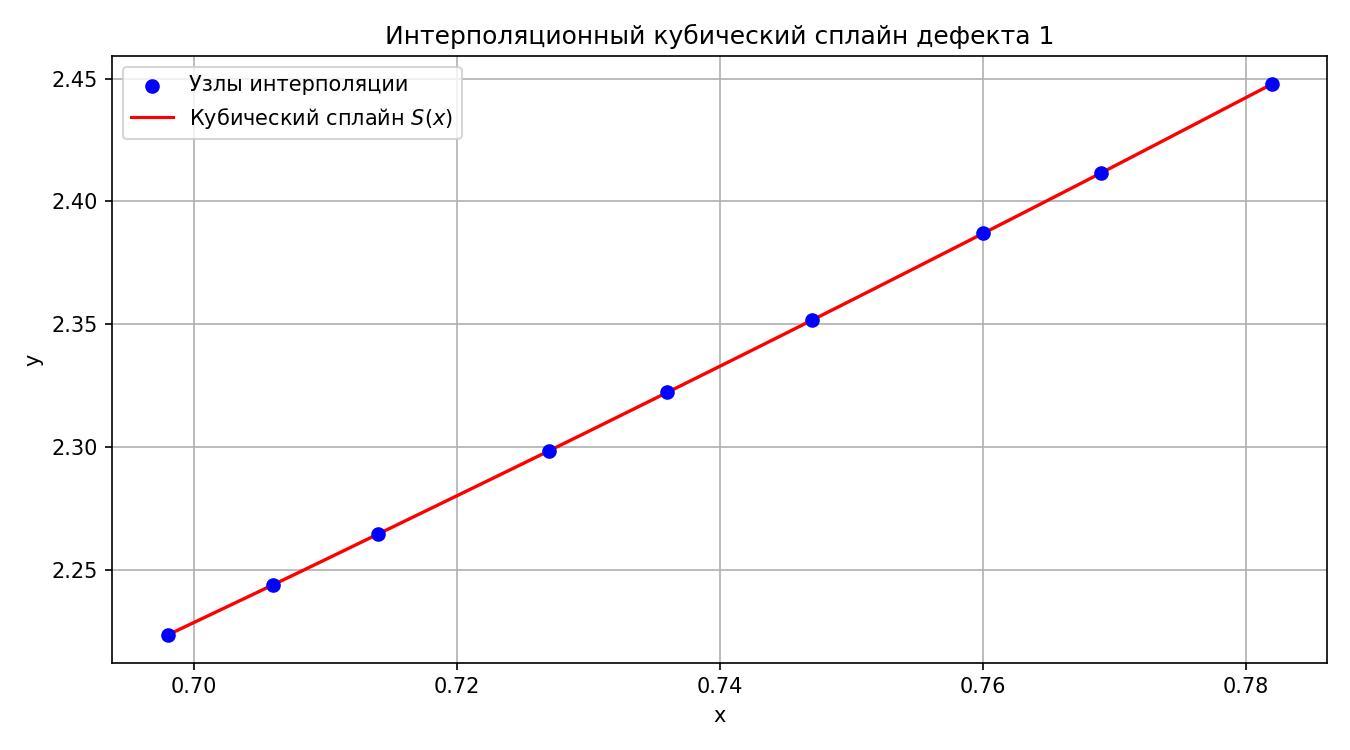
\includegraphics[width=0.9\textwidth]{spline.png}
\caption{Интерполяционный кубический сплайн, построенный по табличной функции.}
\label{fig:spline}
\end{figure}

\newpage

% ============================================================
% conclusion
% ============================================================
\section*{Заключение}
\addcontentsline{toc}{section}{Заключение}

В ходе выполнения лабораторной работы был построен интерполяционный кубический
сплайн дефекта 1 для табличной функции из 9 узлов с граничными условиями на
значение первой производной, оценённой по односторонним разностным формулам.

Граничные наклоны составили $s_0 = 2{,}5500$, $s_8 = 2{,}7846$. Из
трёхдиагональной системы 7 уравнений найдены остальные наклоны
$s_1, \ldots, s_7$. По ним по формуле Эрмита~\eqref{eq:hermite} построены 8
кубических многочленов $P_{3,1}(x), \ldots, P_{3,8}(x)$, составляющих сплайн.

Проведённая проверка показала, что построенный сплайн удовлетворяет всем
налагаемым на него условиям: условиям интерполяции во всех 9 узлах,
непрерывности первой и второй производных во всех 7 внутренних узлах, а также
заданным граничным условиям. Все вычисления выполнены программно на языке
Python с использованием библиотеки NumPy с точностью до четырёх знаков после
запятой в мантиссе.

\end{document}